\documentclass{article}
\usepackage[utf8]{inputenc}
\usepackage{graphicx} % Required for inserting images
\usepackage{float}    % For [H] specifier
\usepackage{caption}  % Better captions
\usepackage{geometry} % Optional: better page margins
\usepackage{subcaption} % For subfigures
\geometry{margin=1in}

\title{}
\author{}
\date{}

\begin{document}

\subsection*{Question 5} \bigskip

\subsubsection*{a) Descriptive Statistics and Boxplots}
\bigskip
The dataset contains 7,687 valid observations of daily demand from four bakery stores in the Vilnius chain. Demand ranges from \textbf{1.02} to \textbf{395.32}, with a mean of \textbf{94.59} and a standard deviation of \textbf{50.93}, which indicates high variability.

\bigskip
\noindent\textbf{Store Observations}

From the data we observe that \emph{Main Street A} has the lowest median demand and a relatively narrow inter quartile range (IQR), but it is also noticeable that there are many irregularities. Since it is the oldest store, this is consistent with its long time series and shows the effects of COVID-related disruptions.

Furthermore, we observe that \emph{Main Street B} has a higher average demand than Main Street A, but with a significantly wider IQR, indicating a larger day-by-day variability. However, this is expected due to its central location and because it was opened after the global pandemic.

Moreover, \emph{Station A} and \emph{Station B} have the highest median demand and the widest IQR's. Their box plots also include long whiskers and many outliers. This could be caused by the variable customer traffic at transportation hubs such as train stations, due to weather, holidays, or tourism cycles.

Finally, in the figure below, on the left side, the box plot for the demand by store is shown. You can see that the variability of demand increases progressively from \emph{Main Street A} to the station locations, with \emph{Main Street B} falling between. 

\bigskip
\noindent\textbf{Weekday Observations}

The data can also be used to analyze the differences in demand across different weekdays. For example, demand tends to increase towards the weekend, as it peaks on \emph{Fridays} and \emph{Saturdays}. 
 In addition, you can see that \emph{Sundays} have the lowest median demand in all stores, with relatively tight distributions.
 Also, from the data, you can see that the demand on the days from \emph{Monday} to \emph{Thursday} maintains consistent levels. They have similar medians and spreads.
 Finally, on the right side of the figure below, the weekday box plots are shown. Here, you can see a rising demand variability on Fridays and Saturdays, particularly in Station A and Main Street A, with Sunday showing much lower and more stable demand.


\begin{figure}[H]
    \centering
    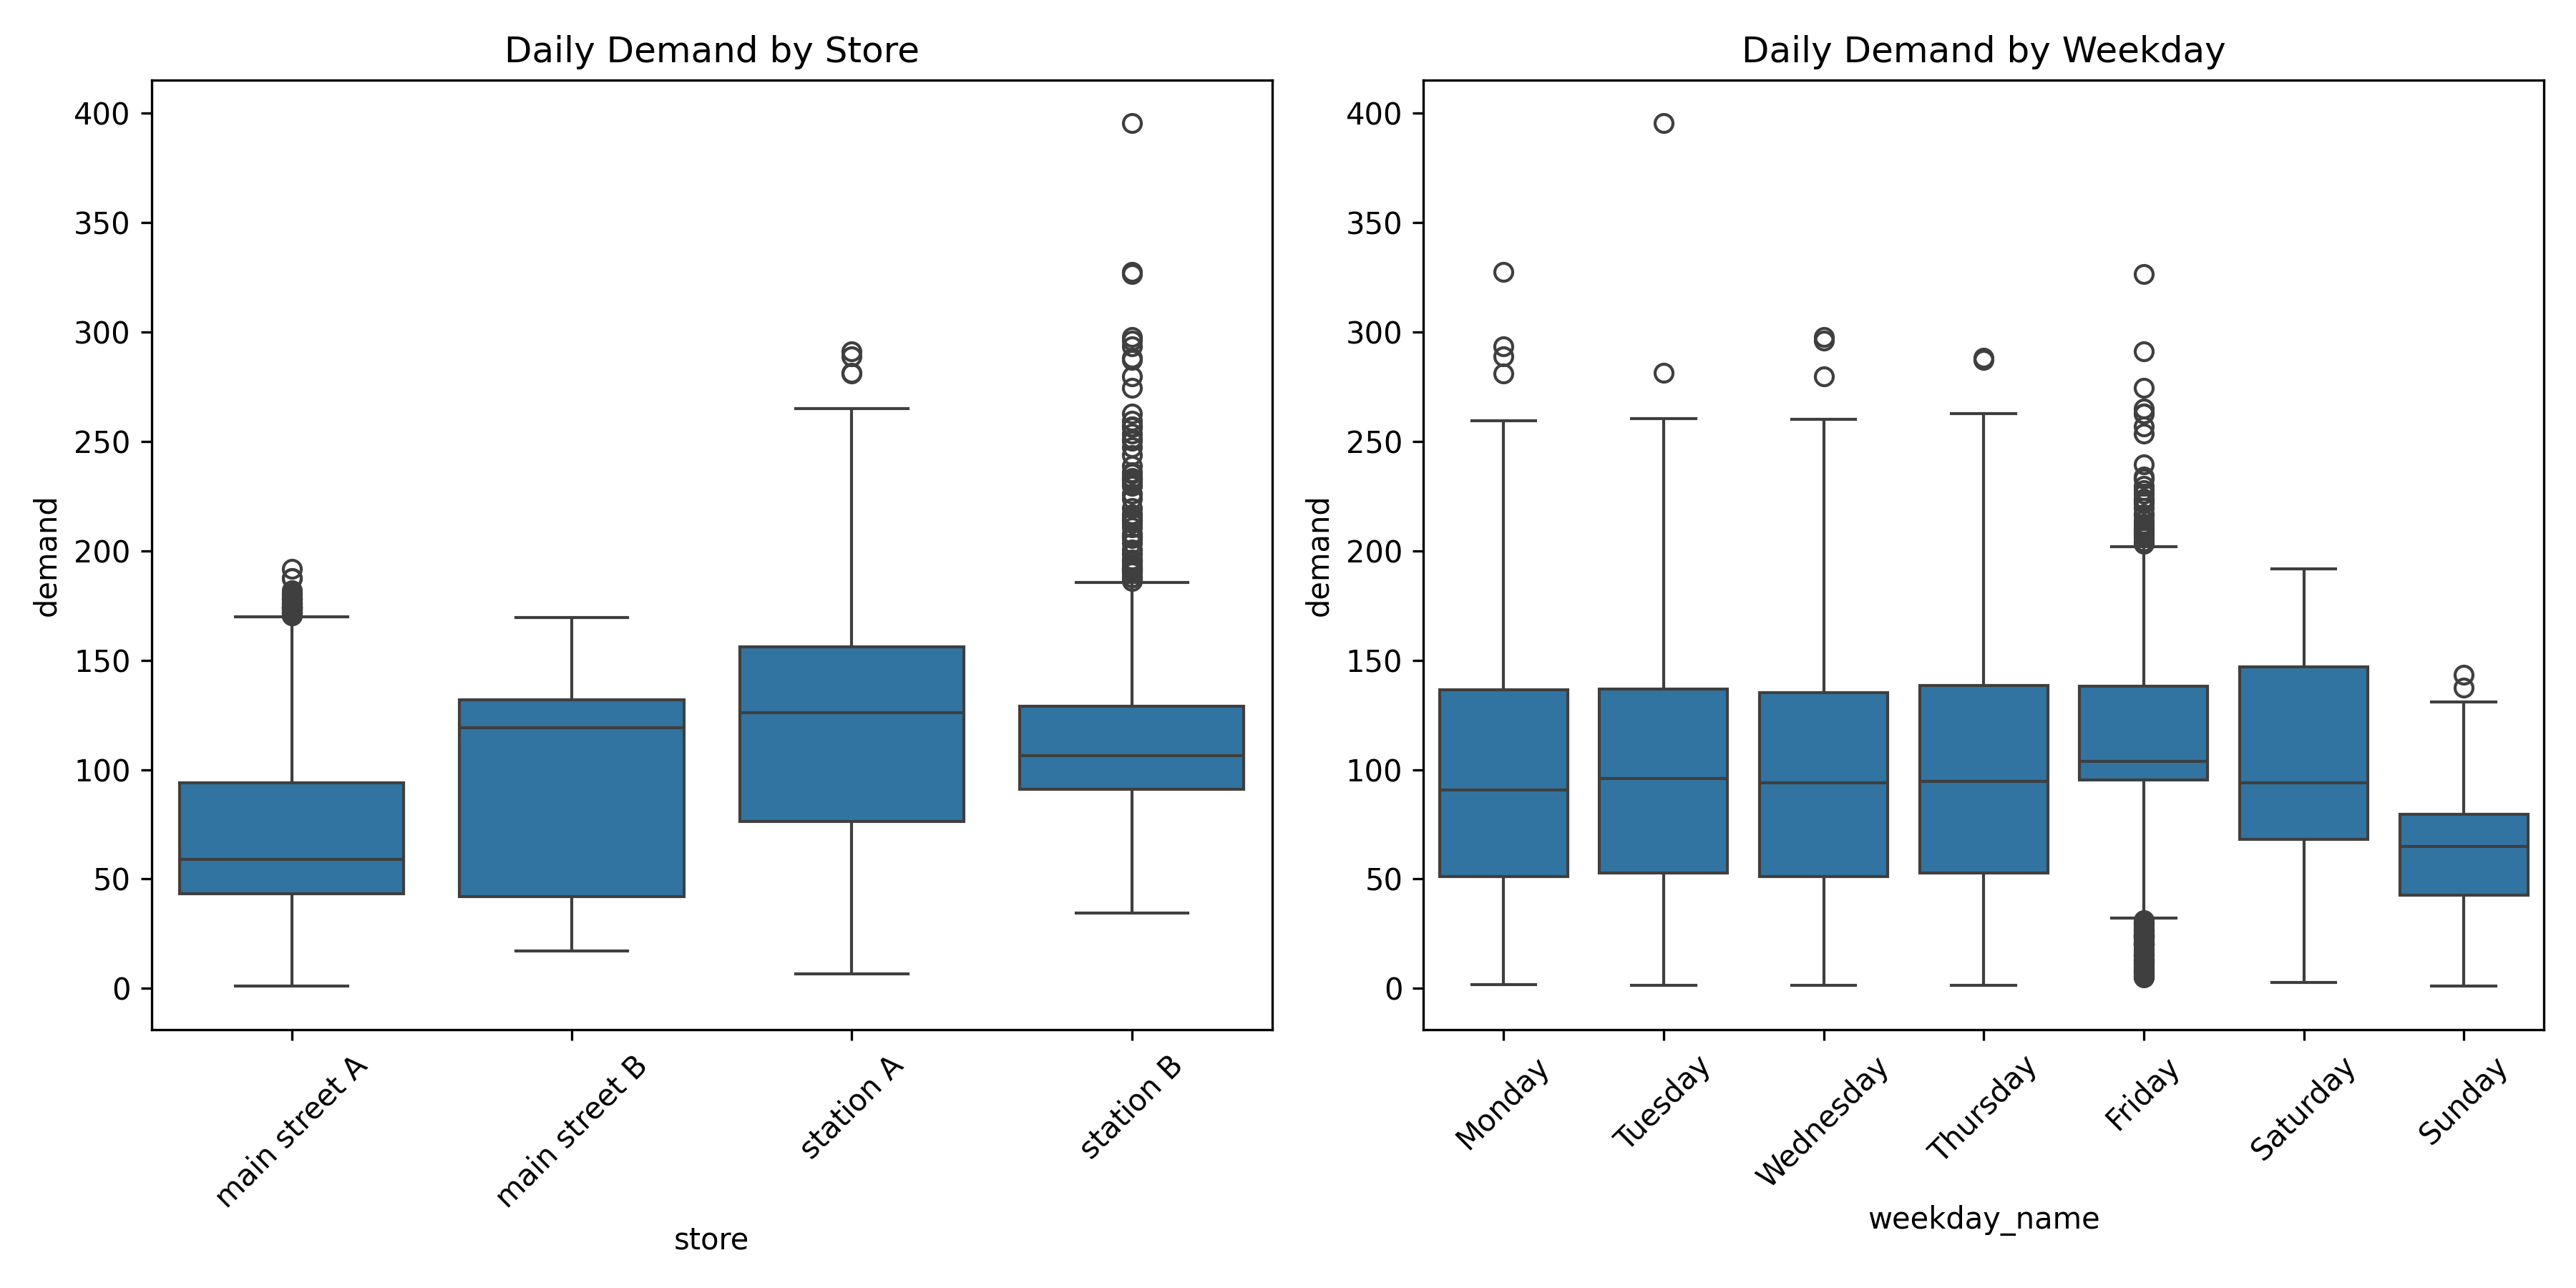
\includegraphics[width=0.95\textwidth]{figures/boxplot_store_and_weekday.png}
    \caption{Boxplot of daily demand per store and by weekday.}
    \label{fig:boxplots}
\end{figure}

\subsubsection*{b) Histograms}
Next, we plot histograms because they provide insight into the distribution of demand for each store. For example, \emph{Main Street A} exhibits a bimodal distribution, likely reflecting the variation of the demand between  weekdays and weekends, as illustrated in Riley et al. (2017), where bimodal demand patterns were observed in stores with different purchase drivers, such as weekly routine shopping versus event or project-based peaks.

Additionally, \emph{Main Street B} shows a milder bimodal pattern, which could possibly be due to the varying demand for workdays and non-workdays. This can also be observed in Riley et al. (2017), where it is discussed how stores serving multiple customer types, such as office workers versus regular passersby, often face split demand distributions.

Furthermore, \emph{Station A} displays a multi-modal and widely spread distribution, indicating inconsistent demand peaks. Kharodawala et al. (2021) highlight that such demand arises in multi-modal supply chains, where the flow is influenced by unpredictable or divided demand sources, like transport hubs or event-based crowd peaks.

Finally, \emph{Station B} has a right-skewed distribution, where most daily demand values group together around a central range, but where a number of days extremely high demand spikes occur. This pattern is typical in locations exposed to irregular spikes in activity, such as transit hubs, where factors like public holidays, tourism, or transport disturbances can lead to sudden and unexpected increases. Rojas et al. (2021) describe how demand skewness causes asymmetry in inventory planning, often requiring a more conservative safety stock level to guard against possible under-stocking on peak days.


\begin{figure}[H]
    \centering
    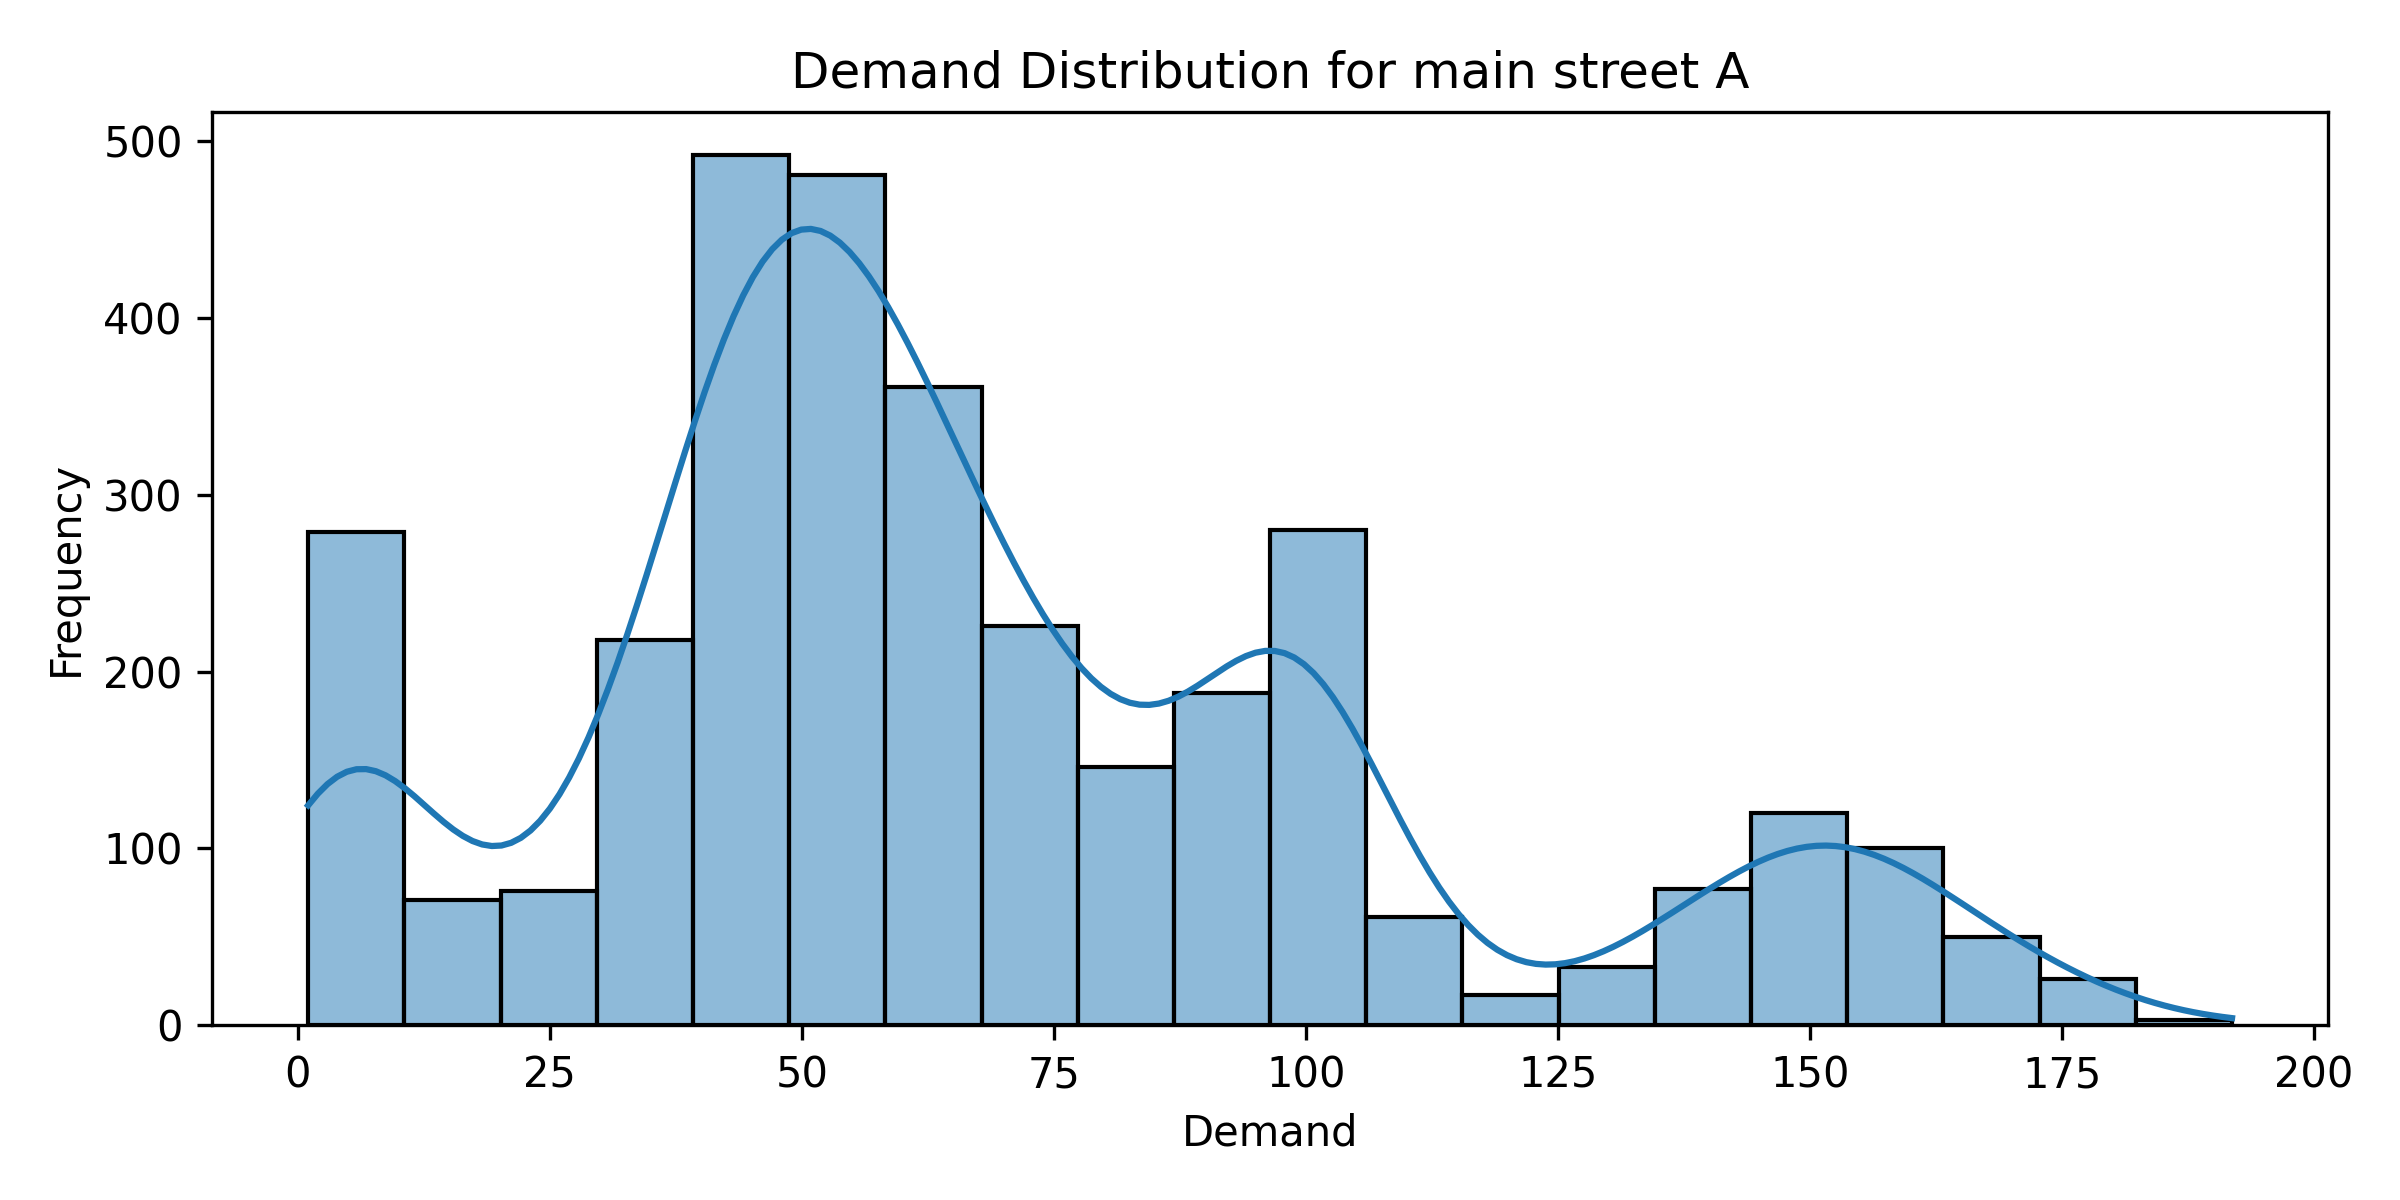
\includegraphics[width=0.49\textwidth]{figures/histogram_main_street_A.png}
    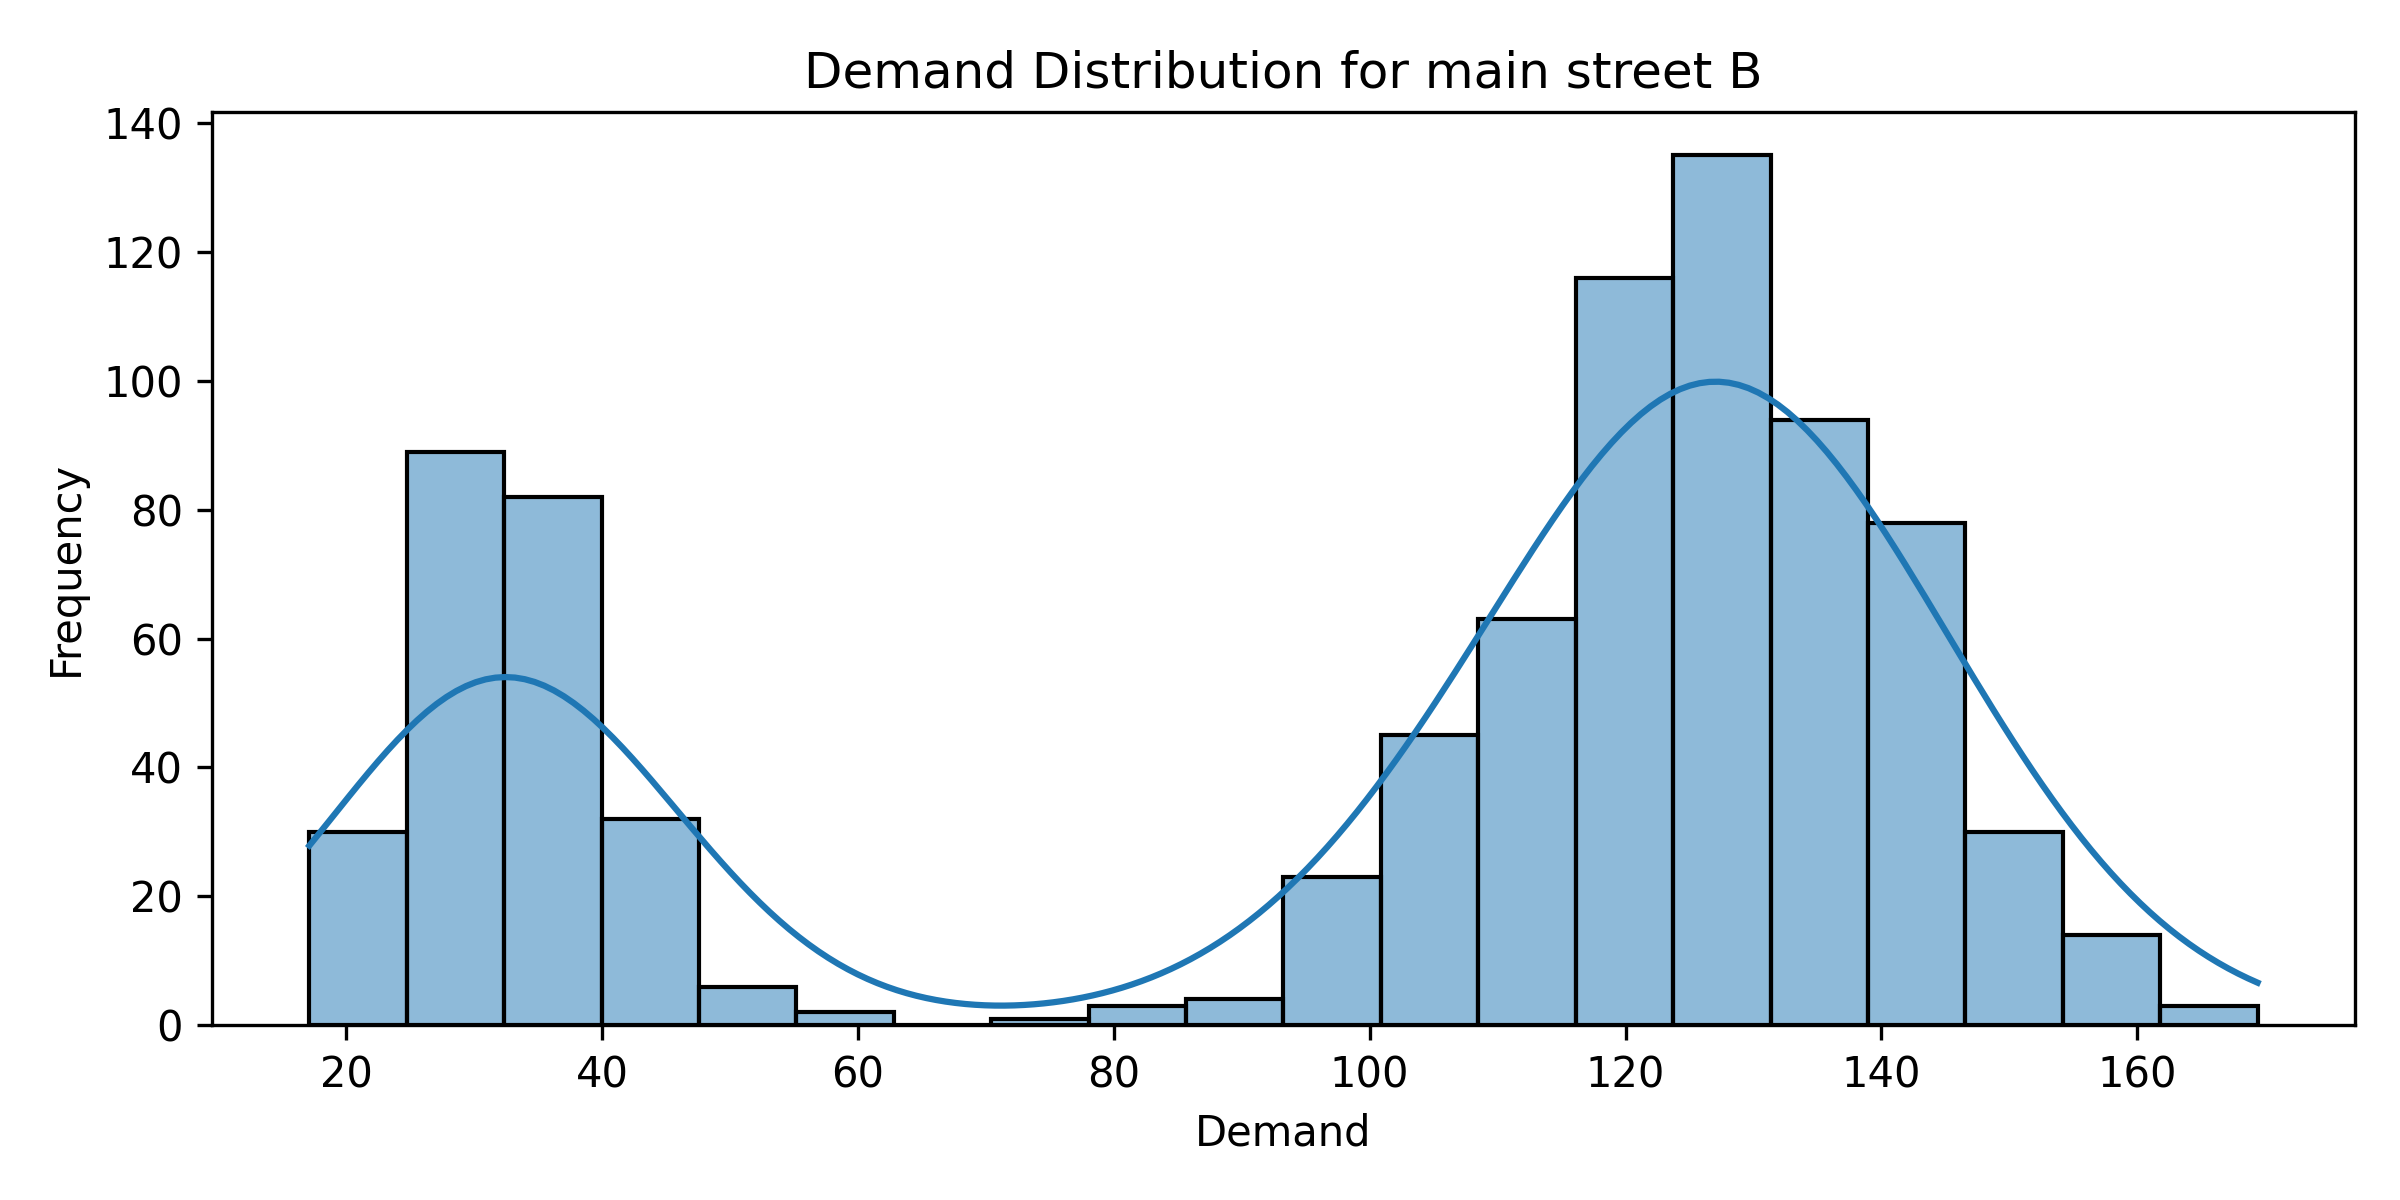
\includegraphics[width=0.49\textwidth]{figures/histogram_main_street_B.png}
    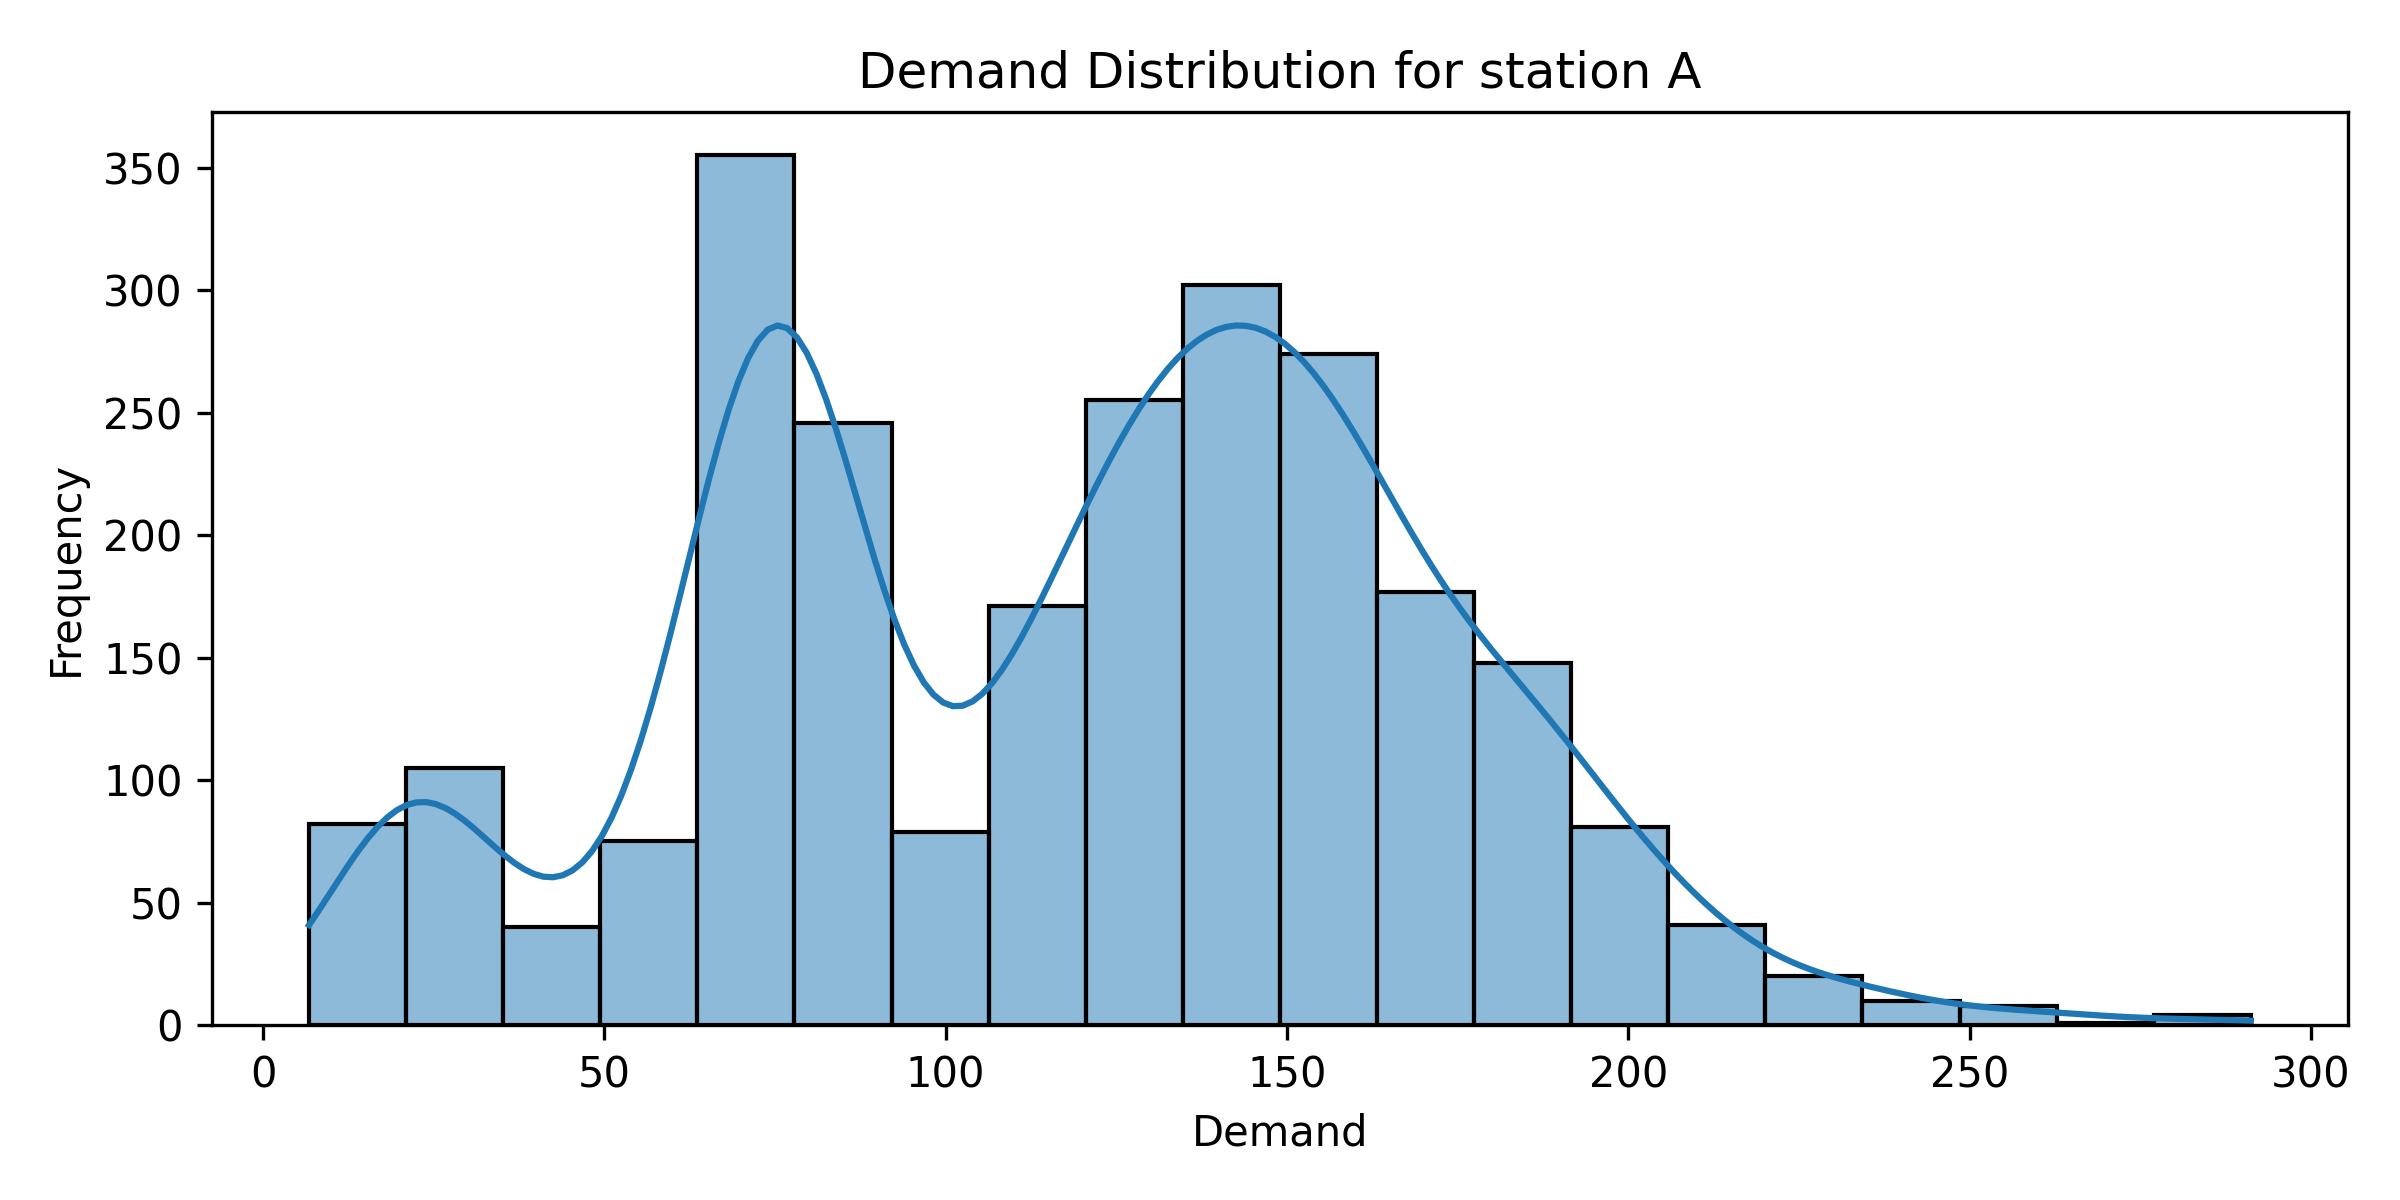
\includegraphics[width=0.49\textwidth]{figures/histogram_station_A.png}
    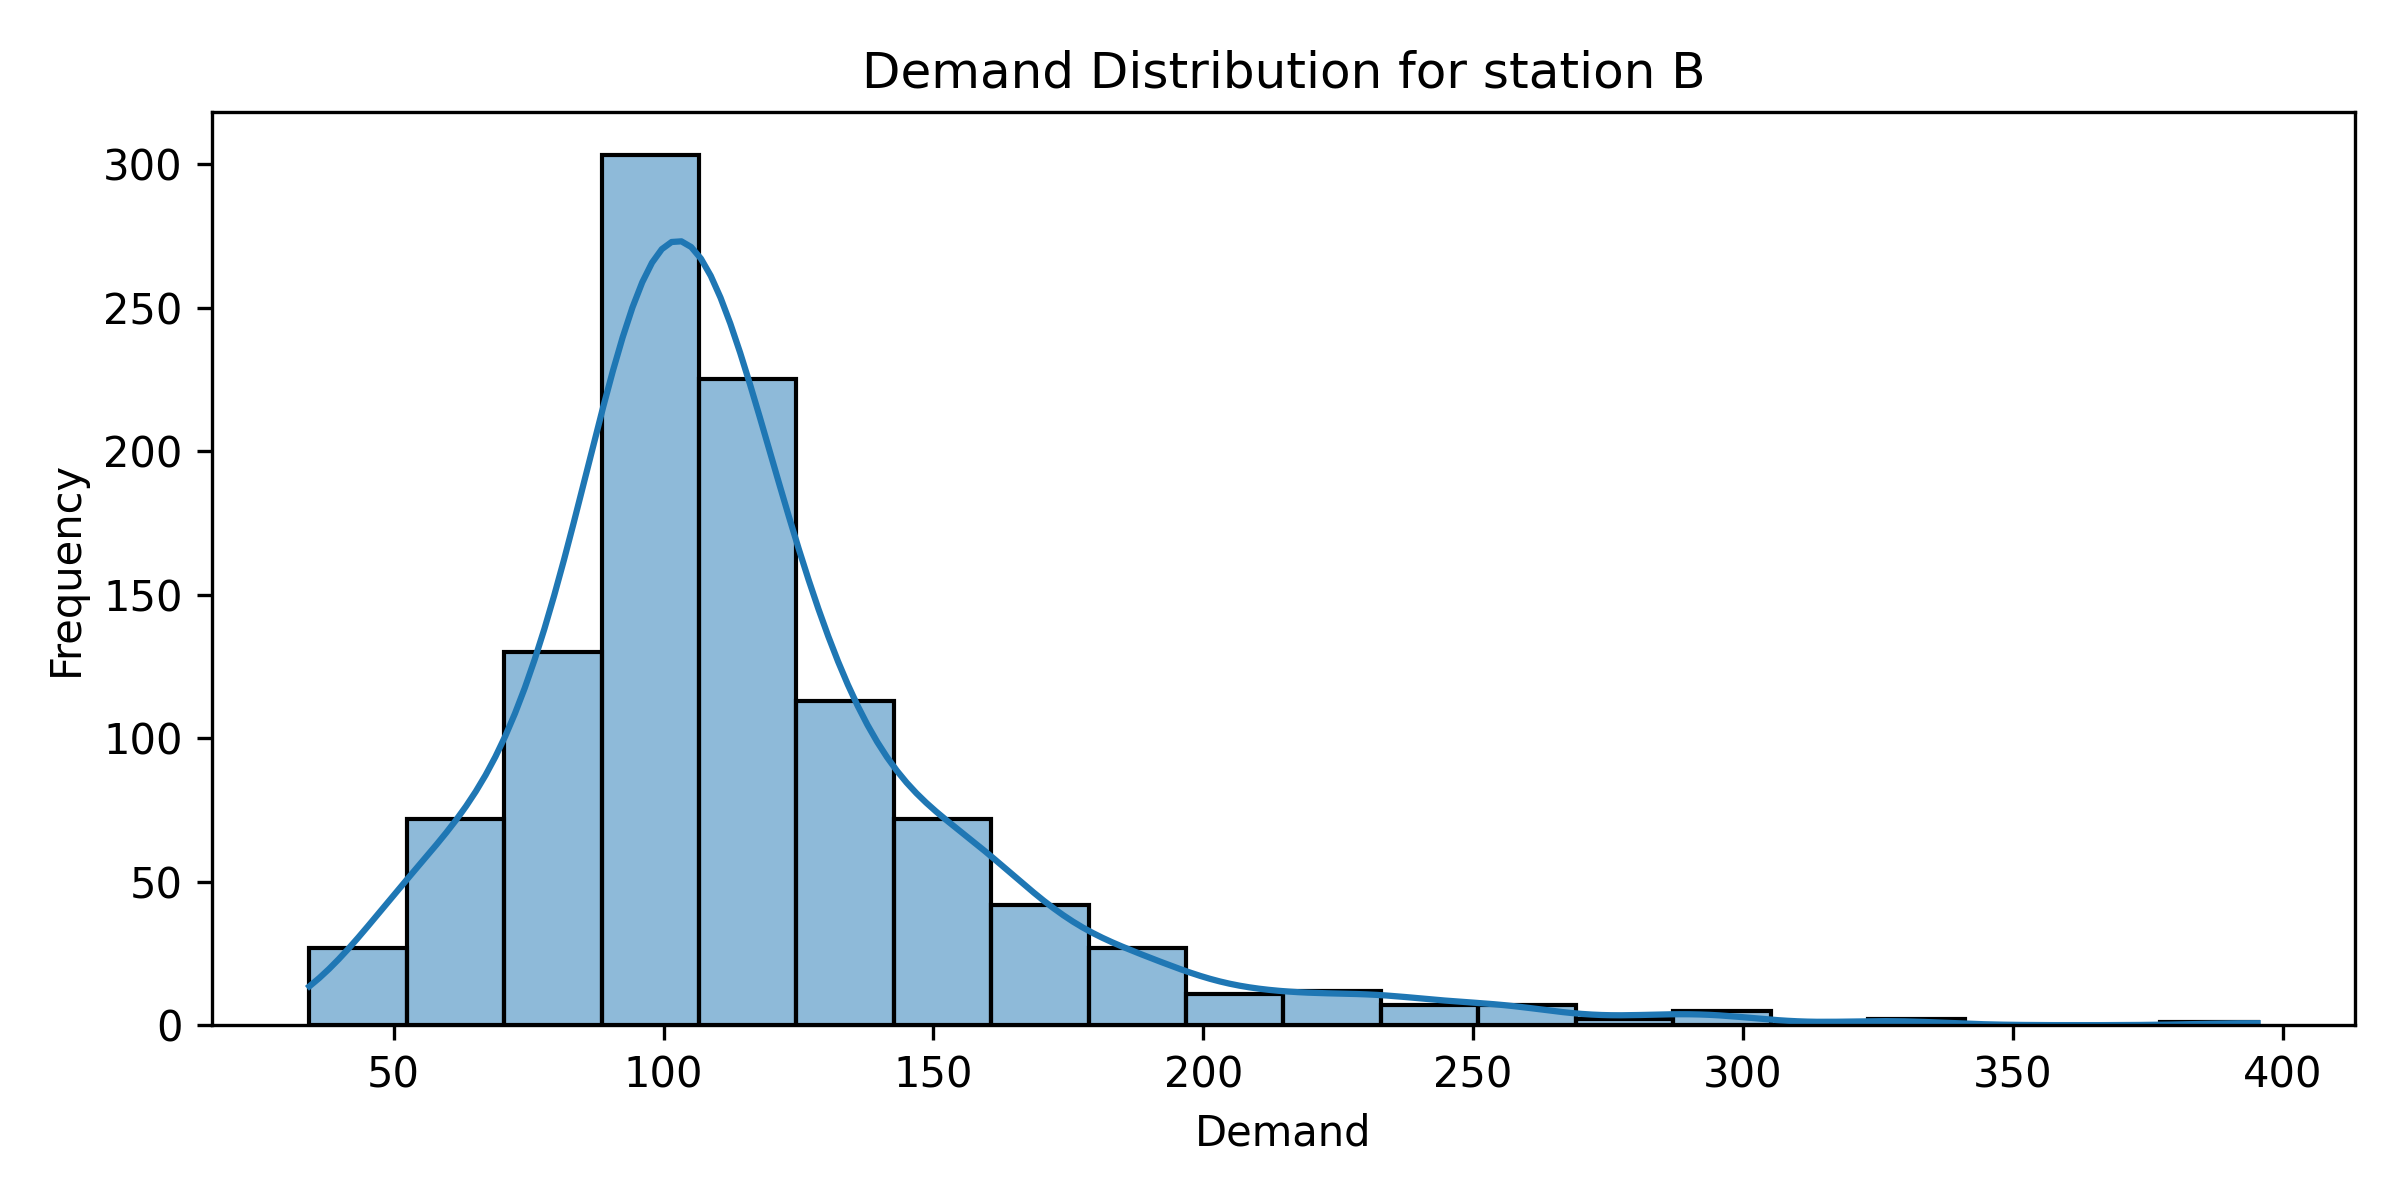
\includegraphics[width=0.49\textwidth]{figures/histogram_station_B.png}
    \caption{Histograms of demand per store.}
    \label{fig:histograms}
\end{figure}

\subsubsection*{c) Time Series Plots}
Below, the time-series plots of the stores are shown, as well as an overlay of the plots in one graph. The time series plots reveal different chronological patterns across stores that reflect on both structural and behavioral incentives of demand. 

%\emph{Main Street A} exhibits a clear COVID-related dip, while newly opened stores show more stable patterns. A weekly cycle with weekend peaks is evident across all stores. 

First, \emph{Main Street A} shows a consistent long-term trend with an obvious dip during the COVID period, followed by a gradual recovery. This pattern shows how disruptive events such as pandemics significantly reduce standard consumer activity, especially in central shopping areas (Rojas et al., 2021).

Second, \emph{Main Street B}, in contrast, shows a regular weekly cycle with little long-term movement, suggesting a stable regular weekday use likely driven by office worker habits. This is consistent with the paper of Riley et al. (2017), since it describes such repeatable demand cycles in shops in business areas, where predictable routines dominate variation.

Third, \emph{Station A} shows long-term high demand with easy observable weekly peaks and periodic peaks, which is consistent with a location highly influenced by transport flow and event-based activity. Kharodawala et al. (2021) note that retail near public transport often experiences multi-modal and unstable demand. This is a pattern that is visible in the station variability and the drop during COVID imitating \emph{Main Street A}.

Finally, \emph{Station B} presents a clearly unstable time series with frequent spikes, but its 7-day average shows a relatively stable trend. This supports the histogram's indication of the right-skewed demand. According to Rojas et al. (2021), this is typical in systems where external shocks, travel behavior, or seasonal effects occasionally raise demand.

As a result, the combined time series plot highlights clear contrasts between stores: the station stores show higher variability and demand peaks, while the main street stores show a smoother and a more regular pattern. The COVID drop is visible in all locations, but its impact was most noticeable in \emph{Main Street A}, highlighting the sensitivity of retail stores in the city to external shocks.




\begin{figure}[H]
    \centering
    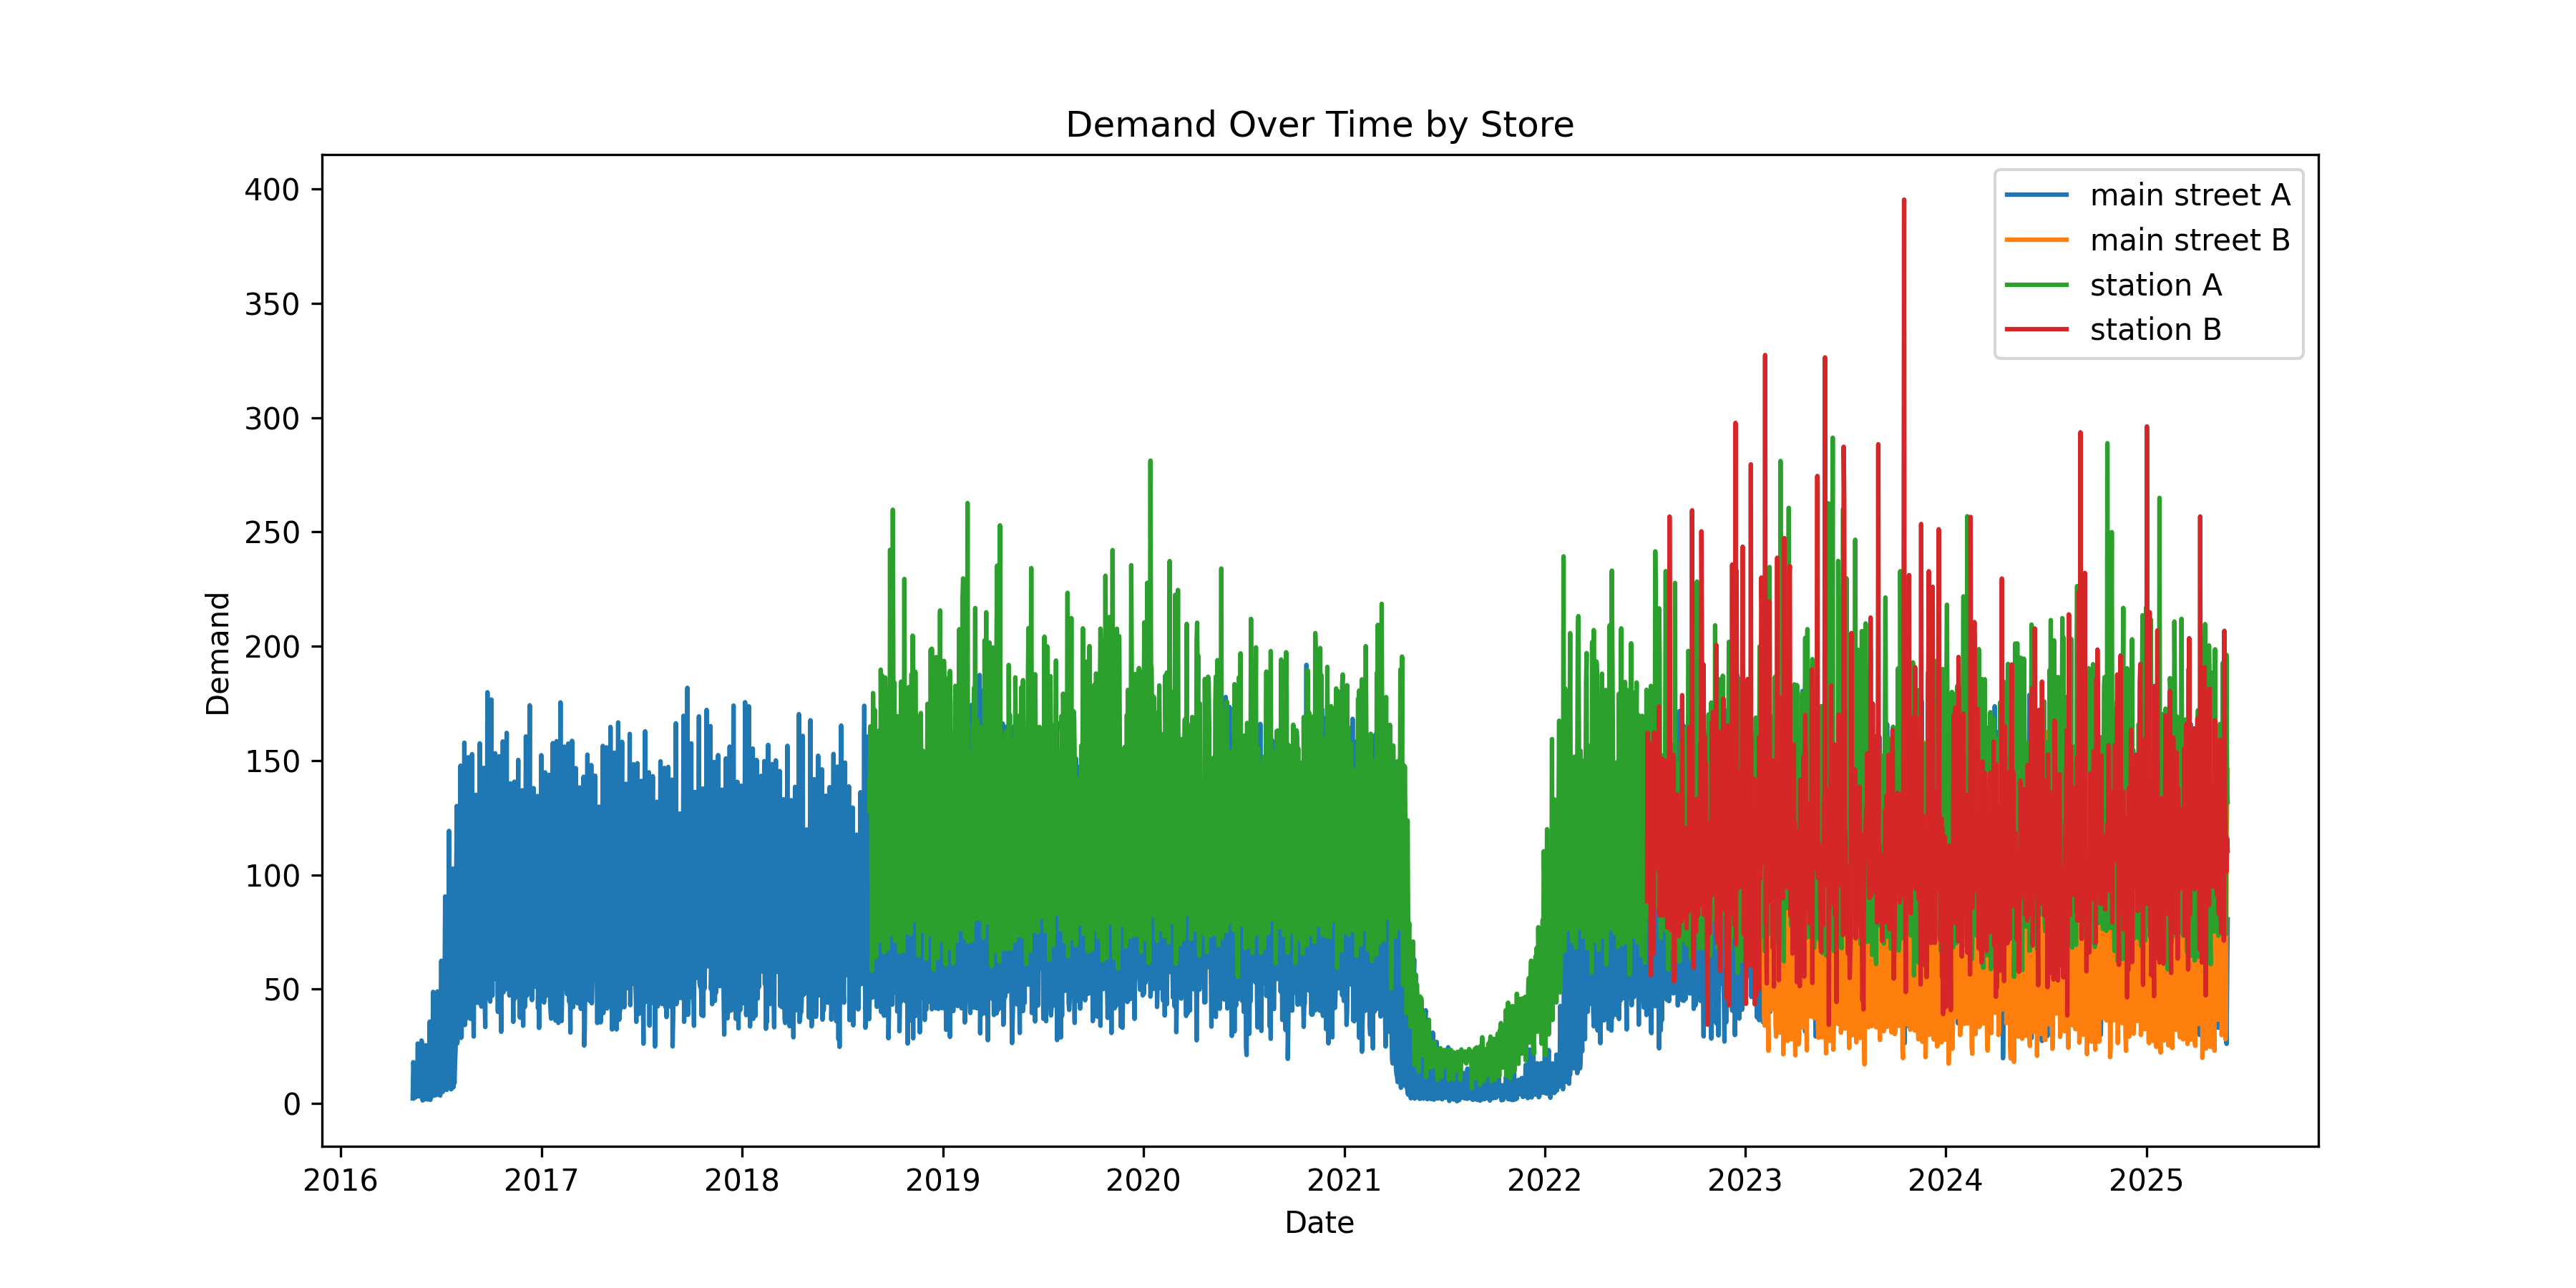
\includegraphics[width=0.95\textwidth]{figures/time_series_all_stores.png}
    \caption{Daily demand over time for all stores.}
    \label{fig:all_timeseries}
\end{figure}

\begin{figure}[H]
    \centering
    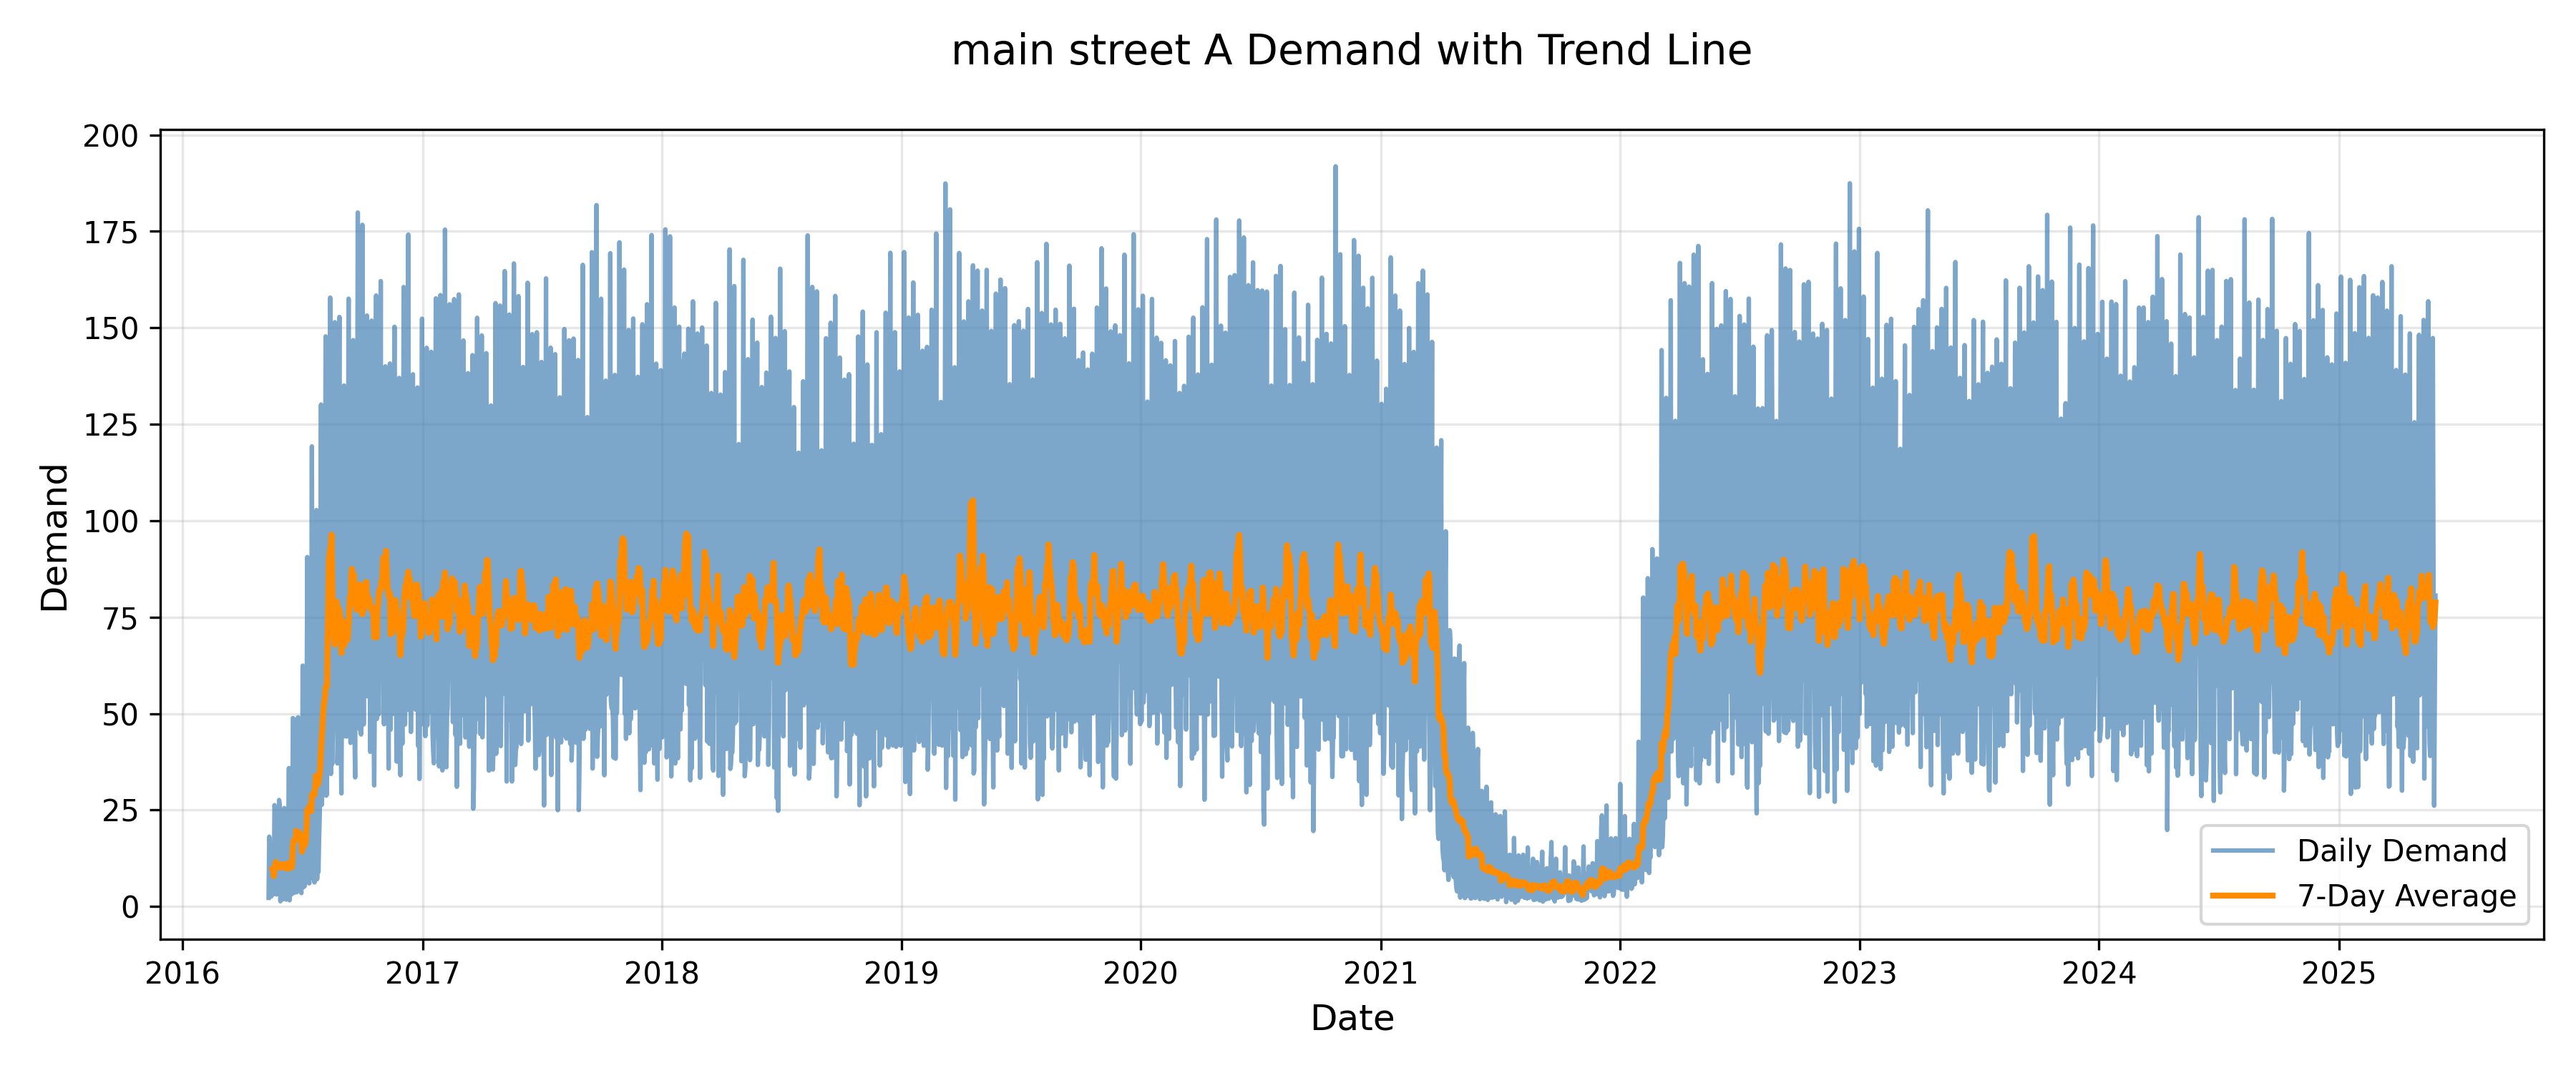
\includegraphics[width=0.48\textwidth]{figures/store_trend_main_street_A.png}
    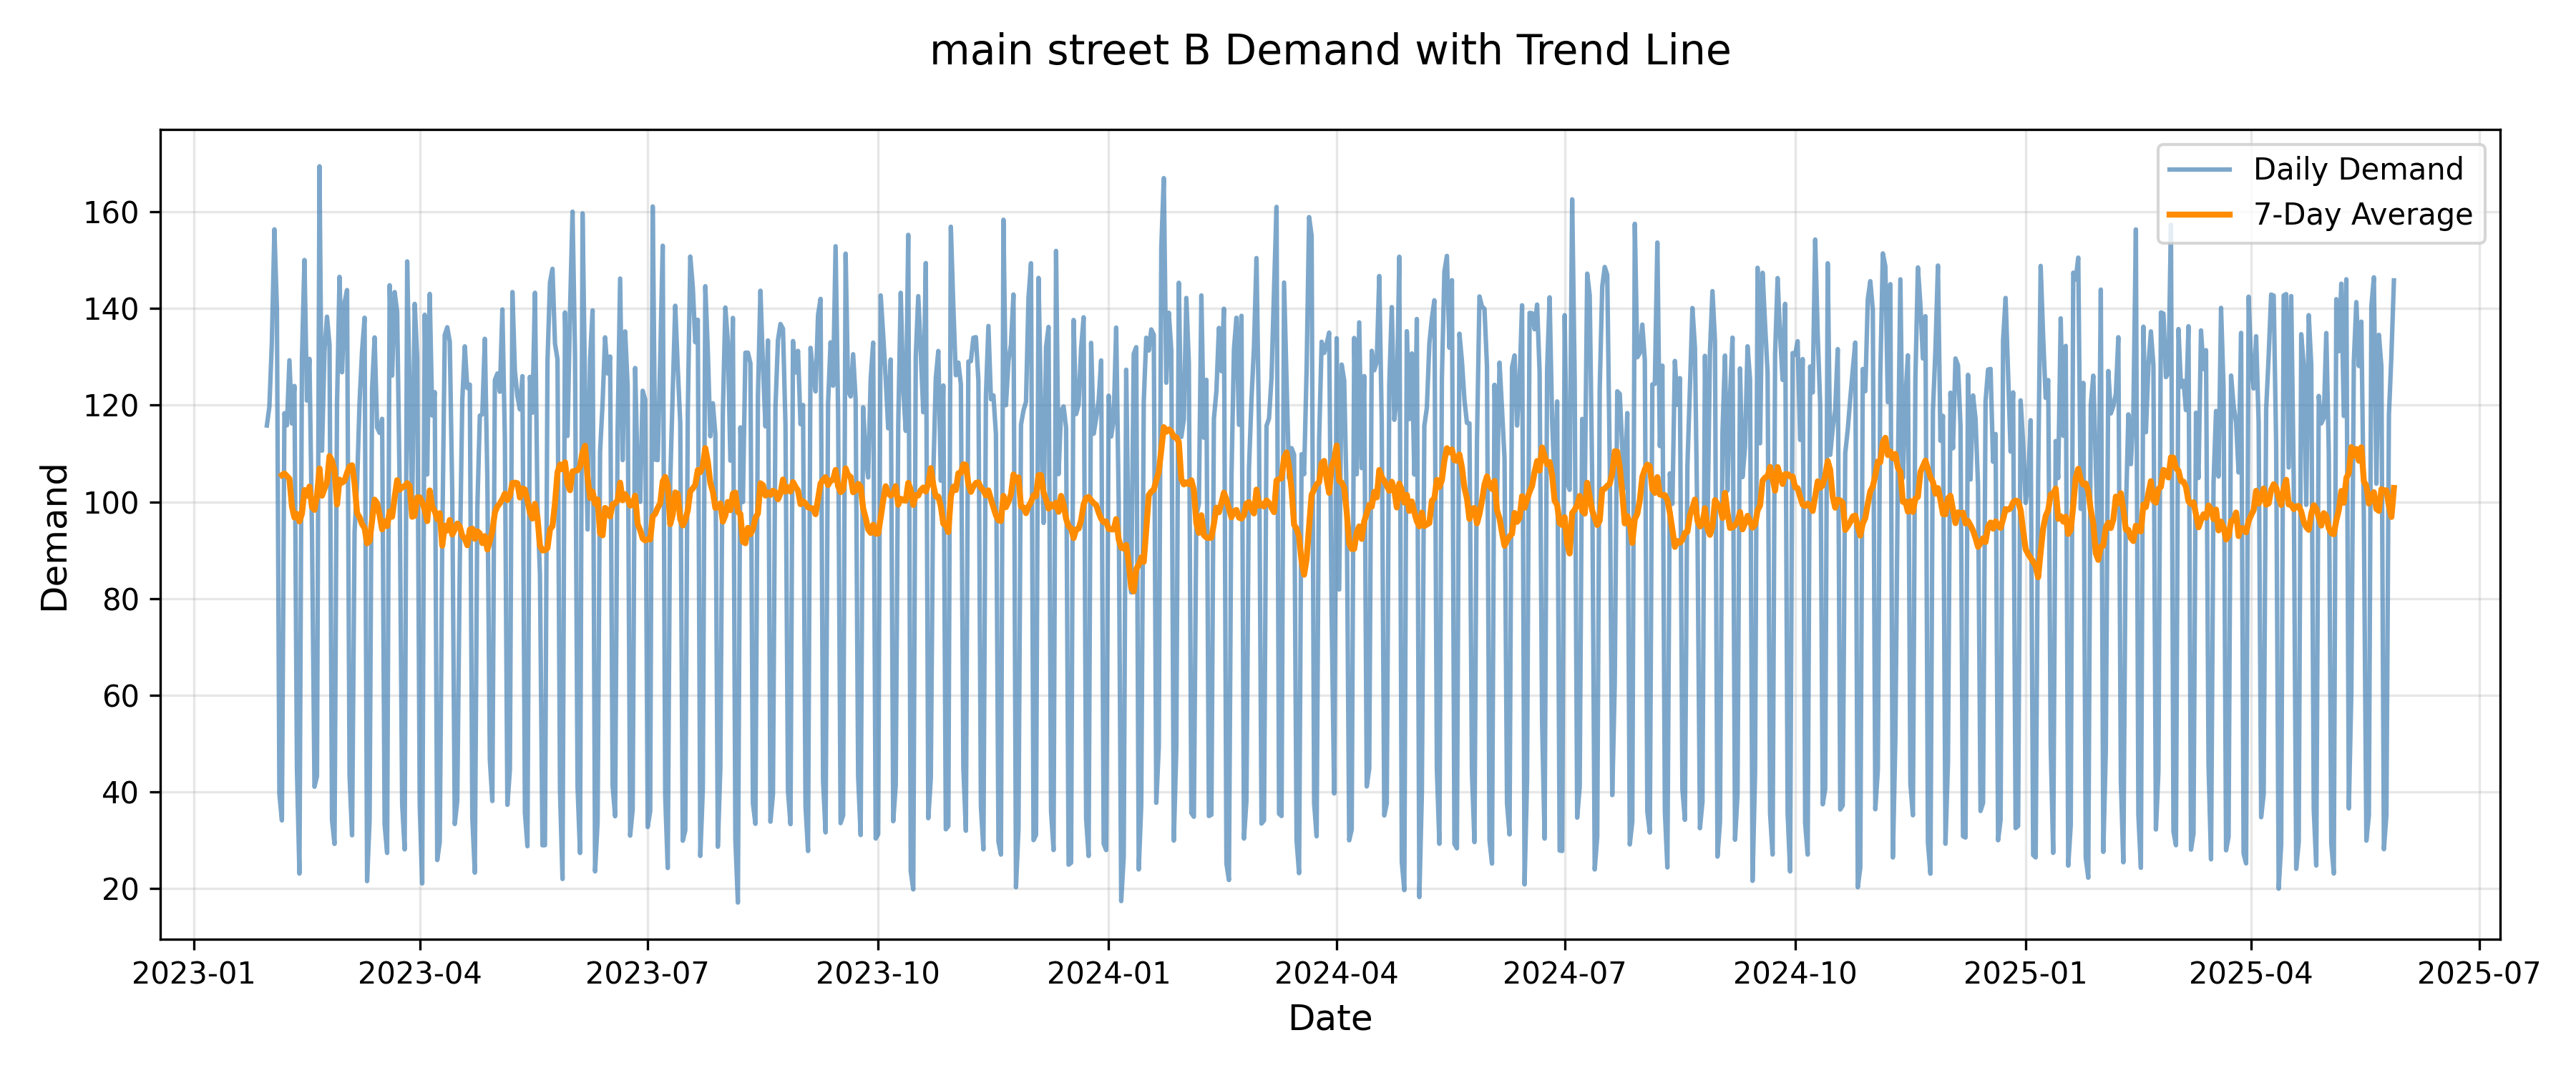
\includegraphics[width=0.48\textwidth]{figures/store_trend_main_street_B.png}
    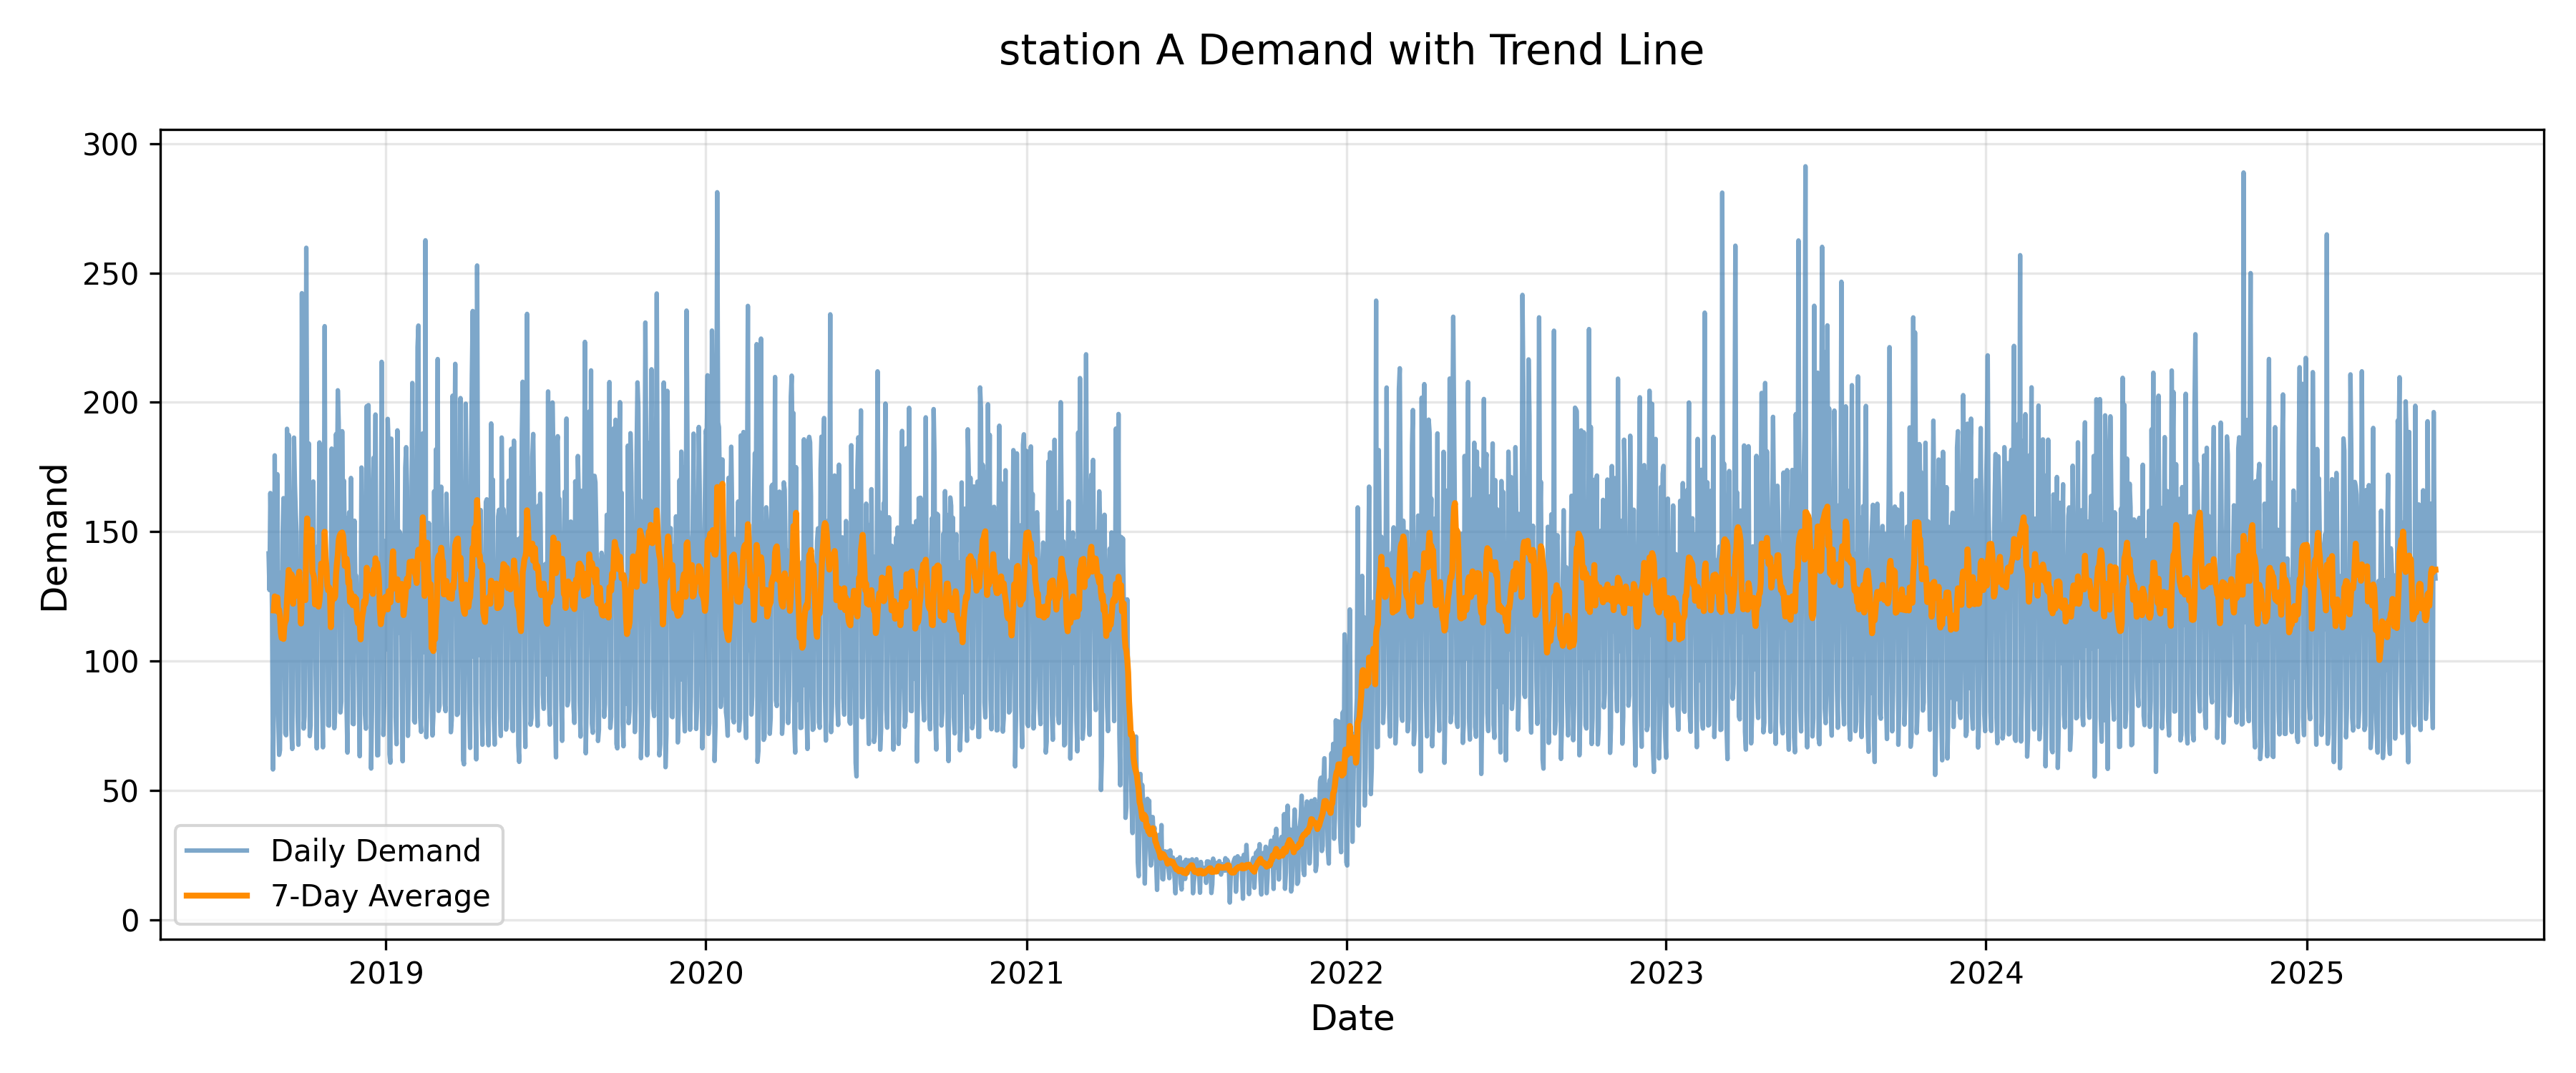
\includegraphics[width=0.48\textwidth]{figures/store_trend_station_A.png}
    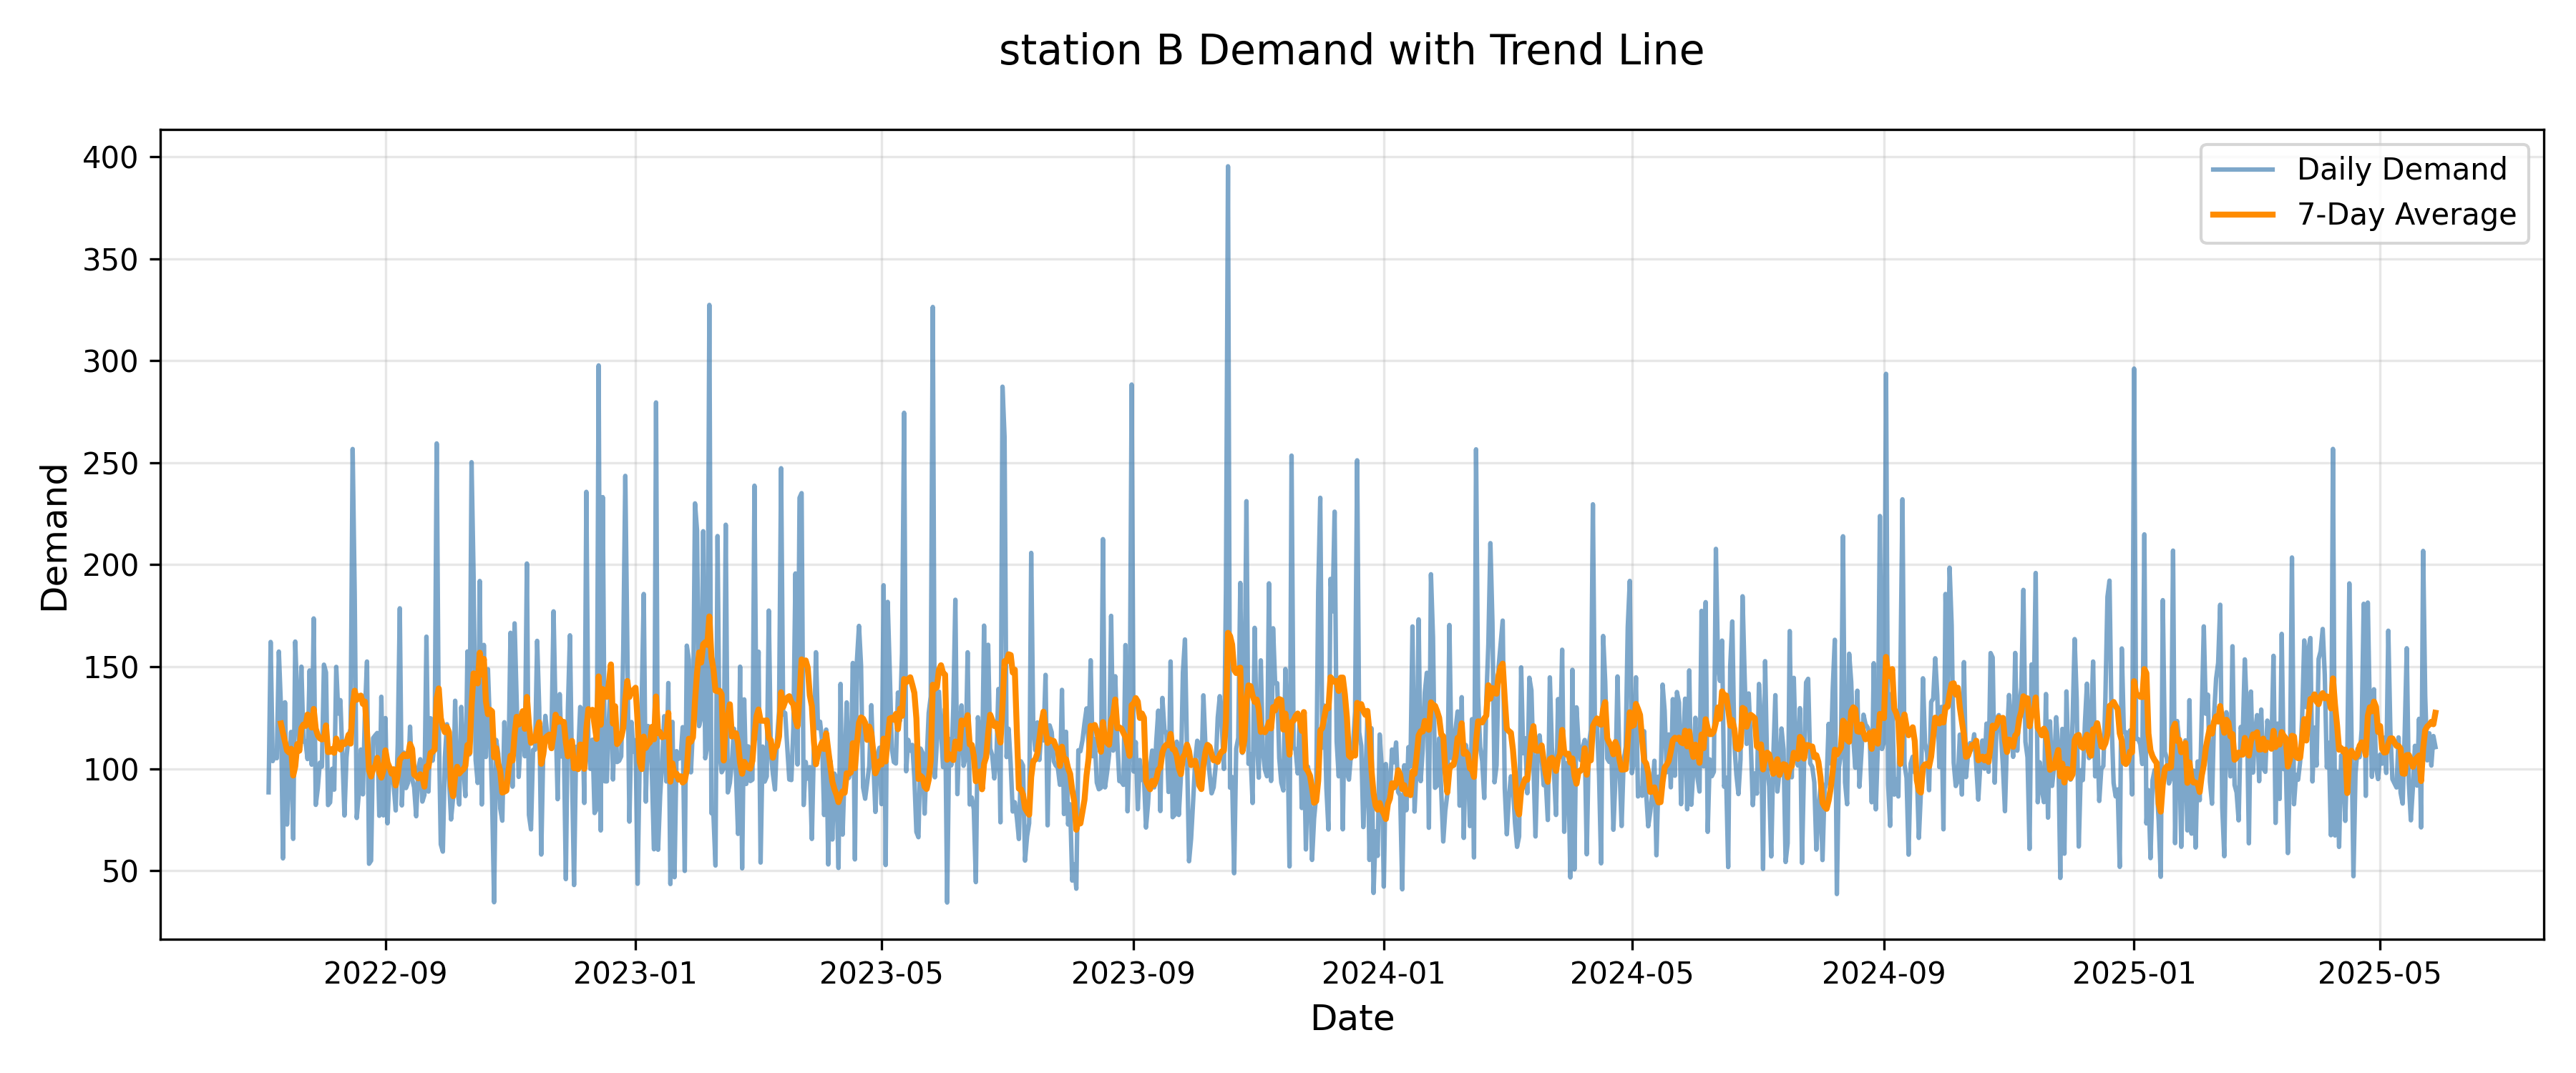
\includegraphics[width=0.48\textwidth]{figures/store_trend_station_B.png}
    \caption{Daily demand and 7-day moving average per store.}
    \label{fig:trend_lines}
\end{figure}

\subsection*{References}

    Kharodawala, H.A., Mahajan, A. \& Moorkanat, J. Multi-modal supply chain distribution problem. OPSEARCH 59, 747–768 (2022). https://doi.org/10.1007/s12597-021-00567-9 

    Riley, J. M., Sweeney, K., Venkataraman, S., \& Klein, R. (2017). How inventory management systems mistreat retail project quantity items and other bimodally distributed products. The International Review Of Retail Distribution And Consumer Research, 28(3), 277–293. https://doi.org/10.1080/09593969.2017.1393442

    Rojas, F., Wanke, P., Bravo, F., \& Tan, Y. (2021). Inventory pooling decisions under demand scenarios in times of COVID-19. Computers \& Industrial Engineering, 161, 107591. https://doi.org/10.1016/j.cie.2021.107591
\end{document}